% Chapter 3

\chapter{Requirements and Methodology} % Main chapter title

\label{Chapter3} % For referencing the chapter elsewhere, use \ref{Chapter1} 

\lhead{Chapter 3. \emph{Requirements and Methodology}}

%----------------------------------------------------------------------------------------

\section{Deliverables}
\label{deliv}

The workload for this MSc project is divided into three different deliverables:

\begin{enumerate}
	\item This research report for the F21RP course (due April 20th).
	\item The MSc thesis report (due August 15th). The report will test the hypotheses listed in Section \ref{reshypo} and draw conclusions from experimental results.
	\item A software package providing implementation of three RL controllers for the F1Tenth platform (due August 15th), detailed in Section \ref{toolimp}.
\end{enumerate}

\section{Research Hypotheses}
\label{reshypo}
I will start by implementing the Wall Following, DQN and DDPG controllers in the F1Tenth simulator. The DQN and DDPG controllers will then be tested on the training race track (the ``RedBull Ring" track from \cite{bosello}), using different sets of hyper-parameters to answer the first hypothesis. Because of a lack of time, the only hyper-parameter that was studied was the reward function; looking at the other hyper-parameters was left as future work. Also because of a lack of time, the DDPG controller wasn't implemented as explained in Chapter \ref{Chapter6}, and the remaining controllers were judged sufficient to test Hypothesis n°1. \\
\textbf{Hypothesis n°1:} \textit{Deep Reinforcement Learning provides a real advantage, quantified by reliable metrics, for controlling an F1Tenth car over human control and PID-based methods like wall following. (Objectives 1,2,3)} \\
To verify the second hypothesis, the performance of the controllers will be compared on the ``RedBull Ring" race track when using a fully connected NN architecture and a CNN. This will be performed in the simulator. \\
\textbf{Hypothesis n°2:} \textit{CNNs offer better results over selected metrics than NNs for autonomous racing on the F1Tenth platform using data from a UST-10LX LiDAR. (Objectives 1,2,3)}\\
To verify the third hypothesis, the three controllers implemented will then be tested on two other race tracks presenting different challenges, namely the ``Silverstone Circuit" and the ``Circuit de Monaco" (both from \cite{bosello}). Those tracks are introduced in Appendix \ref{AppendixA}; importing race tracks has already been tried in the F1Tenth simulator, as explained in Section \ref{preli}. DRL controllers were also trained on the Monaco track to compare their performance with those trained on the RedBull track.\\
\textbf{Hypothesis n°3:} \textit{DRL-based controllers can generalise to new race tracks without affecting the metrics too much. (Objective 3)} \\
With the last hypothesis, I want to evaluate the impact of the gap between the F1Tenth simulator and the real world; developing controllers in the simulator would be useless if they can't be applied to the real world because the gap is too wide. Replicating the complete three circuits in the real world may prove too challenging; in the end, we decided to add a fourth track with an oval shape easier to reproduce in real life, as explained in Chapter \ref{Chapter6}.\\
\textbf{Hypothesis n°4:} \textit{The sim2Real gap is negligible (minor changes of the metrics) and doesn't affect the performance of the controllers implemented. (Objective 5)}\\


\section{Requirements Analysis}
\label{reqana}

The requirements for the project have been divided into experimental requirements (regarding the research hypotheses) presented in Table \ref{expreqtab}, and software requirements presented in Table \ref{softreq}.

\subsection{Experimental Requirements}
\label{expreq}

As will be explained in further detail in Chapter \ref{Chapter6}, because of a lack of time, the experimental requirements (highlighted in Table \ref{expreqtab}) related to the DDPG implementation were dropped, namely requirements E6 and E7.

\begin{table}
\centering
\begin{tabularx}{\textwidth}{||l|X|X|l|l|X||}
 \hline
 Ref & Name & Description & Obj & Priority & State\\ [0.5ex]
 \hline\hline
 E1 & Define a reward function & Define a reward function incentivising safe, smooth and fast car control. & 1 & High & Fully implemented \\
 \hline
 E2 & Implement Wall Following & Implement the Wall Following controller in the simulator, with proper tuning of parameters $k_p$, $k_d$ and $k_i$. & 2 & High & Fully Implemented \\
 \hline
 E3 & Wall Following assessment & Assess the Wall Following controller in the simulator on all three maps (see Appendix \ref{AppendixA}) against selected metrics. & 3 & High & Fully implemented\\
 \hline
 E4 & Implement and train DQN & Implement and train the DQN controller in the simulator with several hyper-parameters and NN architectures. & 2 & High & Fully implemented \\
 \hline
 E5 & DQN assessment & Assess the DQN controller in the simulator on all maps against metrics. & 3 & High & Fully implemented\\ [1ex]
  \hline
 E6 & Implement and train DDPG & Implement and train the DDPG controller with several hyper-parameters and NN architectures. & 2 & Medium & Not implemented\\
  \hline
 E7 & DDPG assessment & Assess DDPG in the simulator on maps against metrics. & 3 & Medium & Not implemented\\ 
 \hline
 E8 & Sim2Real gap assessment & Assess all methods on recreated portions of the 3 maps against metrics; drive the car manually to compare metrics. & 4 & Medium & Partially implemented\\
  \hline
 E9 & Overall Conclusions & Answer all hypotheses. & 5 & High & Fully implemented\\ [1ex]
  \hline
\end{tabularx}
\caption{Experimental Requirements}
\label{expreqtab}
\end{table}

\begin{table}
\centering
\begin{tabularx}{\textwidth}{||l|X|X|l|X||} 
 \hline
 Reference & Name & Description & Priority & Status\\ [0.5ex] 
 \hline\hline
 F1 & Compatibility with F1Tenth platform & The controllers should be easily implementable on the F1Tenth platform & High & Fully implemented\\
 \hline
 F2 & Error Handling & Proper handling of errors in Python & Medium & Partially implemented\\
 \hline
 F3 & Easy parameter change & Let the user specify parameters when launching the .py file; parameters depend on the algorithm chosen. & Low & Fully implemented \\
 \hline
 F4 & Training progress visualisation & Show the user the evolution of the average cumulative reward during the training. & Low & Not implemented\\
 \hline
 F5 &  Logging & For DRL algorithms, states, rewards actions and states should be written in a log file for debugging & Low & Partially implemented\\
 \hline
 F6 &  Implementation with other autonomous car platforms & Basic instructions should be given to implement the controllers on platforms others than F1Tenth & Low & Not implemented\\ [1ex]
 \hline

\end{tabularx}
\caption{Software Requirements}
\label{sofreqtab}
\end{table}

\section{Tooling and Implementation}
\label{toolimp}

A Python codebase will be used to implement this project. The code will be hosted on a public GitHub repository at the URL: \url{https://github.com/HL-Boisvert/MSc_Project_HW}. \newline

The three controllers implemented (Wall Following controller, DQN controller, and DDPG controller) will be available on this GitHub repository, along with their documentation following requirement N1.

The Wall Following controller will be implemented in ROS first and will consist of a single .py file with the following methods and parameters (Figure \ref{wallfollowarch}):

\begin{figure}[H]
\centering
\tikzset{every picture/.style={line width=0.75pt}} %set default line width to 0.75pt        

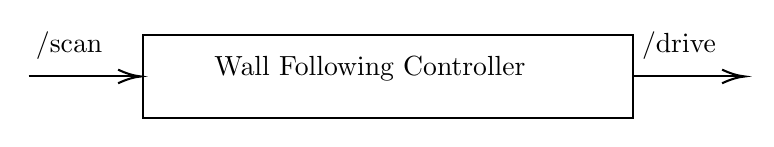
\begin{tikzpicture}[x=0.75pt,y=0.75pt,yscale=-1,xscale=1]
%uncomment if require: \path (0,300); %set diagram left start at 0, and has height of 300

%Shape: Rectangle [id:dp44673081327762776] 
\draw   (208,132) -- (444,132) -- (444,172) -- (208,172) -- cycle ;
%Straight Lines [id:da26472203677837536] 
\draw    (153,152) -- (205,152) ;
\draw [shift={(207,152)}, rotate = 180] [color={rgb, 255:red, 0; green, 0; blue, 0 }  ][line width=0.75]    (10.93,-3.29) .. controls (6.95,-1.4) and (3.31,-0.3) .. (0,0) .. controls (3.31,0.3) and (6.95,1.4) .. (10.93,3.29)   ;
%Straight Lines [id:da8021904942780371] 
\draw    (444,152) -- (496,152) ;
\draw [shift={(498,152)}, rotate = 180] [color={rgb, 255:red, 0; green, 0; blue, 0 }  ][line width=0.75]    (10.93,-3.29) .. controls (6.95,-1.4) and (3.31,-0.3) .. (0,0) .. controls (3.31,0.3) and (6.95,1.4) .. (10.93,3.29)   ;
% Text Node
\draw (241,141) node [anchor=north west][inner sep=0.75pt]   [align=left] {Wall Following Controller};
% Text Node
\draw (155,129) node [anchor=north west][inner sep=0.75pt]   [align=left] {/scan};
% Text Node
\draw (447,129) node [anchor=north west][inner sep=0.75pt]   [align=left] {/drive};
\end{tikzpicture}
\caption{Wall Following controller structure}
\label{wallfollowarch}
\end{figure}

When launching the .py file, the user will have the possibility to specify the $K_p$, $K_i$ and $K_d$ parameters. \newline

Next, the DQN controller will be implemented using a more sophisticated architecture (Figure \ref{dqnarch}).

\begin{figure}[H]
\centering
\tikzset{every picture/.style={line width=0.75pt}} %set default line width to 0.75pt        
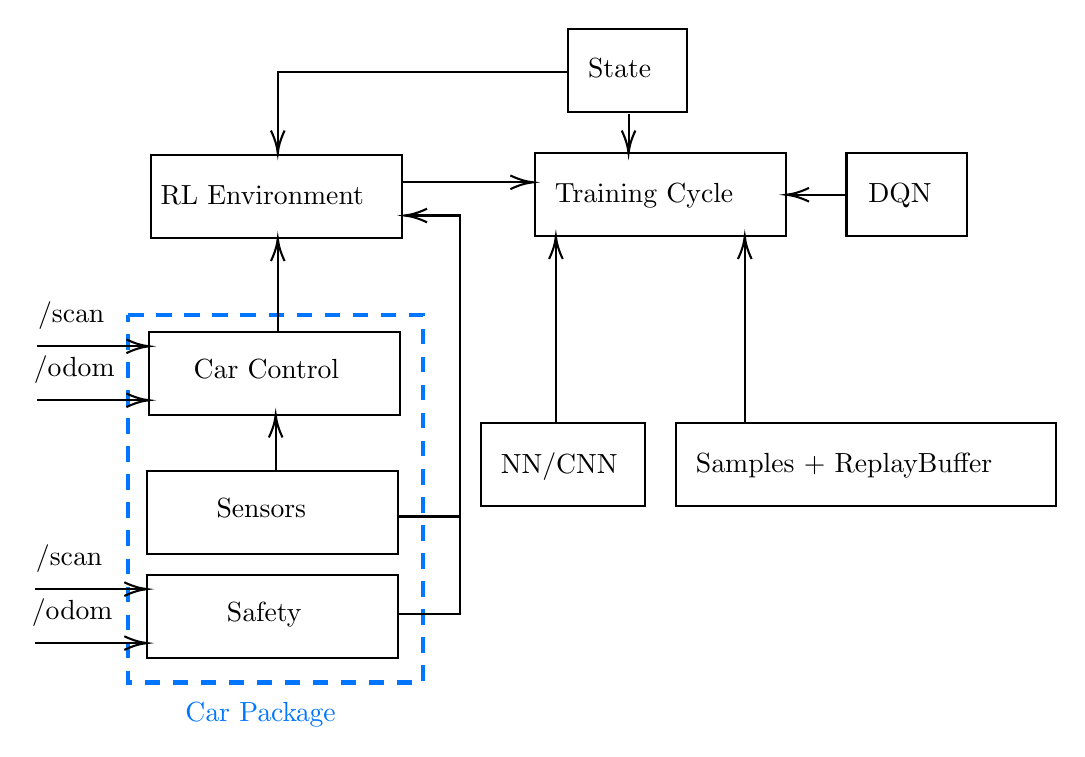
\begin{tikzpicture}[x=0.75pt,y=0.75pt,yscale=-1,xscale=1]
%uncomment if require: \path (0,366); %set diagram left start at 0, and has height of 366

%Shape: Rectangle [id:dp11449840969365366] 
\draw  [color={rgb, 255:red, 0; green, 117; blue, 255 }  ,draw opacity=1 ][dash pattern={on 5.63pt off 4.5pt}][line width=1.5]  (64,149) -- (206.01,149) -- (206.01,326) -- (64,326) -- cycle ;
%Shape: Rectangle [id:dp03081784410716648] 
\draw   (74,157) -- (195,157) -- (195,197) -- (74,197) -- cycle ;
%Shape: Rectangle [id:dp015301803035171702] 
\draw   (73,224) -- (194,224) -- (194,264) -- (73,264) -- cycle ;
%Shape: Rectangle [id:dp42068590308237086] 
\draw   (73,274) -- (194,274) -- (194,314) -- (73,314) -- cycle ;
%Straight Lines [id:da9397976827626164] 
\draw    (19,281) -- (71,281) ;
\draw [shift={(73,281)}, rotate = 180] [color={rgb, 255:red, 0; green, 0; blue, 0 }  ][line width=0.75]    (10.93,-3.29) .. controls (6.95,-1.4) and (3.31,-0.3) .. (0,0) .. controls (3.31,0.3) and (6.95,1.4) .. (10.93,3.29)   ;
%Straight Lines [id:da5105739008906509] 
\draw    (19,307) -- (71,307) ;
\draw [shift={(73,307)}, rotate = 180] [color={rgb, 255:red, 0; green, 0; blue, 0 }  ][line width=0.75]    (10.93,-3.29) .. controls (6.95,-1.4) and (3.31,-0.3) .. (0,0) .. controls (3.31,0.3) and (6.95,1.4) .. (10.93,3.29)   ;
%Straight Lines [id:da40066685510390454] 
\draw    (20,164) -- (72,164) ;
\draw [shift={(74,164)}, rotate = 180] [color={rgb, 255:red, 0; green, 0; blue, 0 }  ][line width=0.75]    (10.93,-3.29) .. controls (6.95,-1.4) and (3.31,-0.3) .. (0,0) .. controls (3.31,0.3) and (6.95,1.4) .. (10.93,3.29)   ;
%Straight Lines [id:da327090026870718] 
\draw    (20,190) -- (72,190) ;
\draw [shift={(74,190)}, rotate = 180] [color={rgb, 255:red, 0; green, 0; blue, 0 }  ][line width=0.75]    (10.93,-3.29) .. controls (6.95,-1.4) and (3.31,-0.3) .. (0,0) .. controls (3.31,0.3) and (6.95,1.4) .. (10.93,3.29)   ;
%Straight Lines [id:da522718763169653] 
\draw    (135,224) -- (135,199) ;
\draw [shift={(135,197)}, rotate = 90] [color={rgb, 255:red, 0; green, 0; blue, 0 }  ][line width=0.75]    (10.93,-3.29) .. controls (6.95,-1.4) and (3.31,-0.3) .. (0,0) .. controls (3.31,0.3) and (6.95,1.4) .. (10.93,3.29)   ;
%Shape: Rectangle [id:dp586400787055392] 
\draw   (75,72) -- (196,72) -- (196,112) -- (75,112) -- cycle ;
%Straight Lines [id:da998544752304739] 
\draw    (136,157) -- (136,114) ;
\draw [shift={(136,112)}, rotate = 90] [color={rgb, 255:red, 0; green, 0; blue, 0 }  ][line width=0.75]    (10.93,-3.29) .. controls (6.95,-1.4) and (3.31,-0.3) .. (0,0) .. controls (3.31,0.3) and (6.95,1.4) .. (10.93,3.29)   ;
%Straight Lines [id:da7916185261016053] 
\draw    (196,85) -- (257,85) ;
\draw [shift={(259,85)}, rotate = 180] [color={rgb, 255:red, 0; green, 0; blue, 0 }  ][line width=0.75]    (10.93,-3.29) .. controls (6.95,-1.4) and (3.31,-0.3) .. (0,0) .. controls (3.31,0.3) and (6.95,1.4) .. (10.93,3.29)   ;
%Straight Lines [id:da9562031880181636] 
\draw    (194,293) -- (224,293) -- (224,101) -- (199,101) ;
\draw [shift={(197,101)}, rotate = 360] [color={rgb, 255:red, 0; green, 0; blue, 0 }  ][line width=0.75]    (10.93,-3.29) .. controls (6.95,-1.4) and (3.31,-0.3) .. (0,0) .. controls (3.31,0.3) and (6.95,1.4) .. (10.93,3.29)   ;
%Straight Lines [id:da8551048605853289] 
\draw    (194,246) -- (224,246) ;
%Shape: Rectangle [id:dp2807542043134432] 
\draw   (260,71) -- (381,71) -- (381,111) -- (260,111) -- cycle ;
%Shape: Rectangle [id:dp3339098892680328] 
\draw   (234,201) -- (313,201) -- (313,241) -- (234,241) -- cycle ;
%Shape: Rectangle [id:dp766870023450984] 
\draw   (410,71) -- (468,71) -- (468,111) -- (410,111) -- cycle ;
%Straight Lines [id:da7117688624558358] 
\draw    (270,201) -- (270,113) ;
\draw [shift={(270,111)}, rotate = 90] [color={rgb, 255:red, 0; green, 0; blue, 0 }  ][line width=0.75]    (10.93,-3.29) .. controls (6.95,-1.4) and (3.31,-0.3) .. (0,0) .. controls (3.31,0.3) and (6.95,1.4) .. (10.93,3.29)   ;
%Straight Lines [id:da6339625502873636] 
\draw    (361,201) -- (361,113) ;
\draw [shift={(361,111)}, rotate = 90] [color={rgb, 255:red, 0; green, 0; blue, 0 }  ][line width=0.75]    (10.93,-3.29) .. controls (6.95,-1.4) and (3.31,-0.3) .. (0,0) .. controls (3.31,0.3) and (6.95,1.4) .. (10.93,3.29)   ;
%Shape: Rectangle [id:dp35618113022054976] 
\draw   (276,11) -- (333,11) -- (333,51) -- (276,51) -- cycle ;
%Straight Lines [id:da336628073889476] 
\draw    (305,52) -- (305,69) ;
\draw [shift={(305,71)}, rotate = 270] [color={rgb, 255:red, 0; green, 0; blue, 0 }  ][line width=0.75]    (10.93,-3.29) .. controls (6.95,-1.4) and (3.31,-0.3) .. (0,0) .. controls (3.31,0.3) and (6.95,1.4) .. (10.93,3.29)   ;
%Straight Lines [id:da3824223244706373] 
\draw    (276,32) -- (136,32) -- (136,69) ;
\draw [shift={(136,71)}, rotate = 270] [color={rgb, 255:red, 0; green, 0; blue, 0 }  ][line width=0.75]    (10.93,-3.29) .. controls (6.95,-1.4) and (3.31,-0.3) .. (0,0) .. controls (3.31,0.3) and (6.95,1.4) .. (10.93,3.29)   ;
%Shape: Rectangle [id:dp2634351109730775] 
\draw   (328,201) -- (511,201) -- (511,241) -- (328,241) -- cycle ;
%Straight Lines [id:da925763979807622] 
\draw    (410,91) -- (383,91) ;
\draw [shift={(381,91)}, rotate = 360] [color={rgb, 255:red, 0; green, 0; blue, 0 }  ][line width=0.75]    (10.93,-3.29) .. controls (6.95,-1.4) and (3.31,-0.3) .. (0,0) .. controls (3.31,0.3) and (6.95,1.4) .. (10.93,3.29)   ;
% Text Node
\draw (94,169) node [anchor=north west][inner sep=0.75pt]   [align=left] {Car Control};
% Text Node
\draw (105,236) node [anchor=north west][inner sep=0.75pt]   [align=left] {Sensors};
% Text Node
\draw (110,286) node [anchor=north west][inner sep=0.75pt]   [align=left] {Safety};
% Text Node
\draw (18,258) node [anchor=north west][inner sep=0.75pt]   [align=left] {/scan};
% Text Node
\draw (16,284) node [anchor=north west][inner sep=0.75pt]   [align=left] {/odom};
% Text Node
\draw (19,141) node [anchor=north west][inner sep=0.75pt]   [align=left] {/scan};
% Text Node
\draw (17,167) node [anchor=north west][inner sep=0.75pt]   [align=left] {/odom};
% Text Node
\draw (78,85) node [anchor=north west][inner sep=0.75pt]   [align=left] {RL Environment};
% Text Node
\draw (268,84) node [anchor=north west][inner sep=0.75pt]   [align=left] {Training Cycle};
% Text Node
\draw (242,214) node [anchor=north west][inner sep=0.75pt]   [align=left] {NN/CNN};
% Text Node
\draw (419,84) node [anchor=north west][inner sep=0.75pt]   [align=left] {DQN};
% Text Node
\draw (284,24) node [anchor=north west][inner sep=0.75pt]   [align=left] {State};
% Text Node
\draw (336,214) node [anchor=north west][inner sep=0.75pt]   [align=left] {Samples + ReplayBuffer};
% Text Node
\draw (90,334) node [anchor=north west][inner sep=0.75pt]   [align=left] {\textcolor[rgb]{0,0.46,1}{Car Package}};
\end{tikzpicture}
\caption{DQN controller structure}
\label{dqnarch}
\end{figure}

The program would be launched in the simulator using the following commands: \\
\verb |$ source devel/setup.bash | \\
\verb |$ roslaunch f1tenth_simulator simulator.launch| \\
\verb |$ python3 training_cycle.py --simulator| \\

The user has the possibility to specify hyper-parameters values (discount, learning rate, maximum number of steps, size of the minibatch sample, NN architecture)  when launching the program using: \\
\verb |$ python3 training_cycle.py --simulator --parameter1=value1 ...| \\
Similar commands are used to launch the controller on the physical car.\\

The DDPG controller will be implemented last, using a similar architecture to the DQN but adding the Actor and Critic classes (Figure \ref{ddpgarchdiagram}):

\begin{figure}[H]
\centering	
\tikzset{every picture/.style={line width=0.75pt}} %set default line width to 0.75pt        
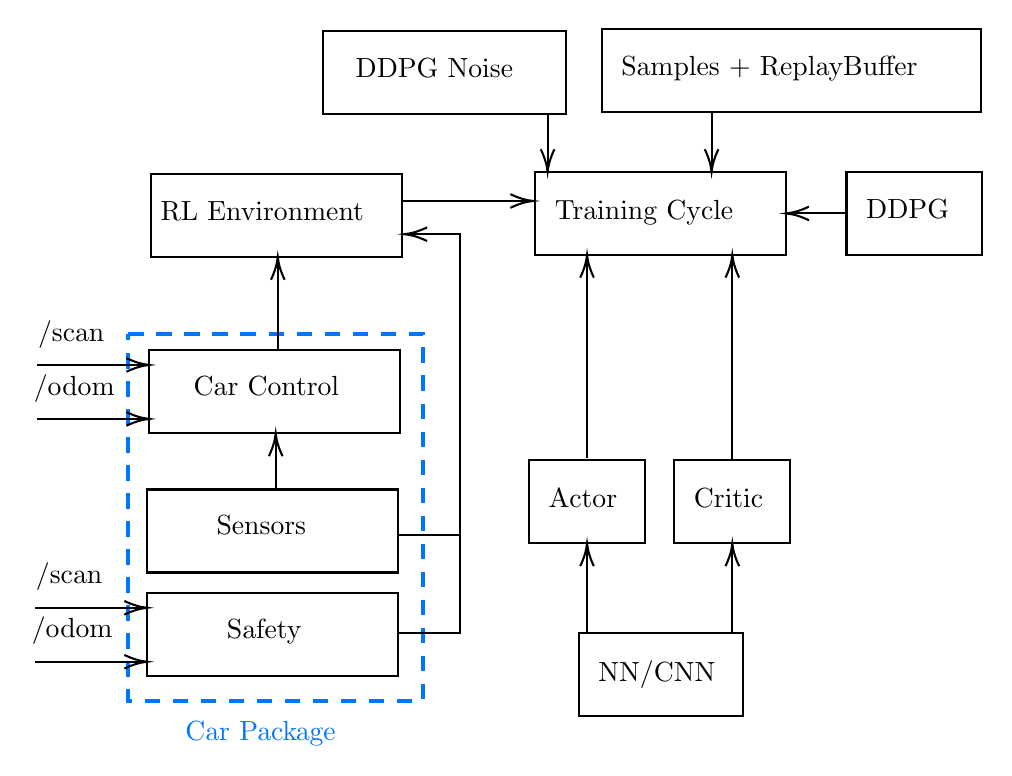
\begin{tikzpicture}[x=0.75pt,y=0.75pt,yscale=-1,xscale=1]
%uncomment if required: \path (0,371); %set diagram left start at 0, and has height of 371
%Shape: Rectangle [id:dp13210929784955172] 
\draw  [color={rgb, 255:red, 0; green, 117; blue, 255 }  ,draw opacity=1 ][dash pattern={on 5.63pt off 4.5pt}][line width=1.5]  (88,160) -- (230.01,160) -- (230.01,337) -- (88,337) -- cycle ;
%Shape: Rectangle [id:dp3003724728725756] 
\draw   (98,168) -- (219,168) -- (219,208) -- (98,208) -- cycle ;
%Shape: Rectangle [id:dp5755918018641251] 
\draw   (97,235) -- (218,235) -- (218,275) -- (97,275) -- cycle ;
%Shape: Rectangle [id:dp9004310636046828] 
\draw   (97,285) -- (218,285) -- (218,325) -- (97,325) -- cycle ;
%Straight Lines [id:da45790386241122394] 
\draw    (43,292) -- (95,292) ;
\draw [shift={(97,292)}, rotate = 180] [color={rgb, 255:red, 0; green, 0; blue, 0 }  ][line width=0.75]    (10.93,-3.29) .. controls (6.95,-1.4) and (3.31,-0.3) .. (0,0) .. controls (3.31,0.3) and (6.95,1.4) .. (10.93,3.29)   ;
%Straight Lines [id:da3258136216670251] 
\draw    (43,318) -- (95,318) ;
\draw [shift={(97,318)}, rotate = 180] [color={rgb, 255:red, 0; green, 0; blue, 0 }  ][line width=0.75]    (10.93,-3.29) .. controls (6.95,-1.4) and (3.31,-0.3) .. (0,0) .. controls (3.31,0.3) and (6.95,1.4) .. (10.93,3.29)   ;
%Straight Lines [id:da1014073191407956] 
\draw    (44,175) -- (96,175) ;
\draw [shift={(98,175)}, rotate = 180] [color={rgb, 255:red, 0; green, 0; blue, 0 }  ][line width=0.75]    (10.93,-3.29) .. controls (6.95,-1.4) and (3.31,-0.3) .. (0,0) .. controls (3.31,0.3) and (6.95,1.4) .. (10.93,3.29)   ;
%Straight Lines [id:da9203574215098338] 
\draw    (44,201) -- (96,201) ;
\draw [shift={(98,201)}, rotate = 180] [color={rgb, 255:red, 0; green, 0; blue, 0 }  ][line width=0.75]    (10.93,-3.29) .. controls (6.95,-1.4) and (3.31,-0.3) .. (0,0) .. controls (3.31,0.3) and (6.95,1.4) .. (10.93,3.29)   ;
%Straight Lines [id:da6394991063845095] 
\draw    (159,235) -- (159,210) ;
\draw [shift={(159,208)}, rotate = 90] [color={rgb, 255:red, 0; green, 0; blue, 0 }  ][line width=0.75]    (10.93,-3.29) .. controls (6.95,-1.4) and (3.31,-0.3) .. (0,0) .. controls (3.31,0.3) and (6.95,1.4) .. (10.93,3.29)   ;
%Shape: Rectangle [id:dp9916576994435125] 
\draw   (99,83) -- (220,83) -- (220,123) -- (99,123) -- cycle ;
%Straight Lines [id:da04342321560868645] 
\draw    (160,168) -- (160,125) ;
\draw [shift={(160,123)}, rotate = 90] [color={rgb, 255:red, 0; green, 0; blue, 0 }  ][line width=0.75]    (10.93,-3.29) .. controls (6.95,-1.4) and (3.31,-0.3) .. (0,0) .. controls (3.31,0.3) and (6.95,1.4) .. (10.93,3.29)   ;
%Straight Lines [id:da20917400871366798] 
\draw    (220,96) -- (281,96) ;
\draw [shift={(283,96)}, rotate = 180] [color={rgb, 255:red, 0; green, 0; blue, 0 }  ][line width=0.75]    (10.93,-3.29) .. controls (6.95,-1.4) and (3.31,-0.3) .. (0,0) .. controls (3.31,0.3) and (6.95,1.4) .. (10.93,3.29)   ;
%Straight Lines [id:da30459802757031107] 
\draw    (218,304) -- (248,304) -- (248,112) -- (223,112) ;
\draw [shift={(221,112)}, rotate = 360] [color={rgb, 255:red, 0; green, 0; blue, 0 }  ][line width=0.75]    (10.93,-3.29) .. controls (6.95,-1.4) and (3.31,-0.3) .. (0,0) .. controls (3.31,0.3) and (6.95,1.4) .. (10.93,3.29)   ;
%Straight Lines [id:da14904241185621414] 
\draw    (218,257) -- (248,257) ;
%Shape: Rectangle [id:dp905443614389843] 
\draw   (284,82) -- (405,82) -- (405,122) -- (284,122) -- cycle ;
%Shape: Rectangle [id:dp7989214721219287] 
\draw   (305,304) -- (384,304) -- (384,344) -- (305,344) -- cycle ;
%Shape: Rectangle [id:dp5109388425513526] 
\draw   (434,82) -- (499.5,82) -- (499.5,122) -- (434,122) -- cycle ;
%Straight Lines [id:da5263046961940592] 
\draw    (309,220) -- (309,124) ;
\draw [shift={(309,122)}, rotate = 90] [color={rgb, 255:red, 0; green, 0; blue, 0 }  ][line width=0.75]    (10.93,-3.29) .. controls (6.95,-1.4) and (3.31,-0.3) .. (0,0) .. controls (3.31,0.3) and (6.95,1.4) .. (10.93,3.29)   ;
%Straight Lines [id:da016883730956527954] 
\draw    (379,221) -- (379,124) ;
\draw [shift={(379,122)}, rotate = 90] [color={rgb, 255:red, 0; green, 0; blue, 0 }  ][line width=0.75]    (10.93,-3.29) .. controls (6.95,-1.4) and (3.31,-0.3) .. (0,0) .. controls (3.31,0.3) and (6.95,1.4) .. (10.93,3.29)   ;
%Shape: Rectangle [id:dp7992865547214365] 
\draw   (316,13) -- (499,13) -- (499,53) -- (316,53) -- cycle ;
%Straight Lines [id:da7956509261955109] 
\draw    (434,102) -- (407,102) ;
\draw [shift={(405,102)}, rotate = 360] [color={rgb, 255:red, 0; green, 0; blue, 0 }  ][line width=0.75]    (10.93,-3.29) .. controls (6.95,-1.4) and (3.31,-0.3) .. (0,0) .. controls (3.31,0.3) and (6.95,1.4) .. (10.93,3.29)   ;
%Straight Lines [id:da833793752029848] 
\draw    (369,53) -- (369,80) ;
\draw [shift={(369,82)}, rotate = 270] [color={rgb, 255:red, 0; green, 0; blue, 0 }  ][line width=0.75]    (10.93,-3.29) .. controls (6.95,-1.4) and (3.31,-0.3) .. (0,0) .. controls (3.31,0.3) and (6.95,1.4) .. (10.93,3.29)   ;
%Shape: Rectangle [id:dp4764150239534557] 
\draw   (281,221) -- (337,221) -- (337,261) -- (281,261) -- cycle ;
%Shape: Rectangle [id:dp7625399319432427] 
\draw   (351,221) -- (407,221) -- (407,261) -- (351,261) -- cycle ;
%Straight Lines [id:da6270527667010888] 
\draw    (309,303.57) -- (309,263) ;
\draw [shift={(309,261)}, rotate = 90] [color={rgb, 255:red, 0; green, 0; blue, 0 }  ][line width=0.75]    (10.93,-3.29) .. controls (6.95,-1.4) and (3.31,-0.3) .. (0,0) .. controls (3.31,0.3) and (6.95,1.4) .. (10.93,3.29)   ;
%Straight Lines [id:da5325466952436175] 
\draw    (379,304) -- (379,263) ;
\draw [shift={(379,261)}, rotate = 90] [color={rgb, 255:red, 0; green, 0; blue, 0 }  ][line width=0.75]    (10.93,-3.29) .. controls (6.95,-1.4) and (3.31,-0.3) .. (0,0) .. controls (3.31,0.3) and (6.95,1.4) .. (10.93,3.29)   ;
%Shape: Rectangle [id:dp8140292645454428] 
\draw   (182,14) -- (299,14) -- (299,54) -- (182,54) -- cycle ;
%Straight Lines [id:da32430121666514755] 
\draw    (290,54) -- (290,80) ;
\draw [shift={(290,82)}, rotate = 270] [color={rgb, 255:red, 0; green, 0; blue, 0 }  ][line width=0.75]    (10.93,-3.29) .. controls (6.95,-1.4) and (3.31,-0.3) .. (0,0) .. controls (3.31,0.3) and (6.95,1.4) .. (10.93,3.29)   ;
% Text Node
\draw (118,179) node [anchor=north west][inner sep=0.75pt]   [align=left] {Car Control};
% Text Node
\draw (129,246) node [anchor=north west][inner sep=0.75pt]   [align=left] {Sensors};
% Text Node
\draw (134,296) node [anchor=north west][inner sep=0.75pt]   [align=left] {Safety};
% Text Node
\draw (42,269) node [anchor=north west][inner sep=0.75pt]   [align=left] {/scan};
% Text Node
\draw (40,295) node [anchor=north west][inner sep=0.75pt]   [align=left] {/odom};
% Text Node
\draw (43,152) node [anchor=north west][inner sep=0.75pt]   [align=left] {/scan};
% Text Node
\draw (41,178) node [anchor=north west][inner sep=0.75pt]   [align=left] {/odom};
% Text Node
\draw (102,95) node [anchor=north west][inner sep=0.75pt]   [align=left] {RL Environment};
% Text Node
\draw (292,94) node [anchor=north west][inner sep=0.75pt]   [align=left] {Training Cycle};
% Text Node
\draw (313,316) node [anchor=north west][inner sep=0.75pt]   [align=left] {NN/CNN};
% Text Node
\draw (442,94) node [anchor=north west][inner sep=0.75pt]   [align=left] {DDPG};
% Text Node
\draw (324,25) node [anchor=north west][inner sep=0.75pt]   [align=left] {Samples + ReplayBuffer};
% Text Node
\draw (114,345) node [anchor=north west][inner sep=0.75pt]   [align=left] {\textcolor[rgb]{0,0.46,1}{Car Package}};
% Text Node
\draw (289,233) node [anchor=north west][inner sep=0.75pt]   [align=left] {Actor};
% Text Node
\draw (359,233) node [anchor=north west][inner sep=0.75pt]   [align=left] {Critic};
% Text Node
\draw (196,26) node [anchor=north west][inner sep=0.75pt]   [align=left] {DDPG Noise};
\end{tikzpicture}
\caption{DDPG controller structure}
\label{ddpgarchdiagram}
\end{figure}

The agent inputs and outputs for both the DQN and DDPG controllers are as introduced in Figure \ref{inputs_outputs}. The data from the \verb|\odom| and \verb|\scan| topics is obtained through the \verb|get_car_state()| function, then is processed and stored in a state. The state stored in the replay memory is then fed to the \verb|behavior_predict(state)| function, which returns an array of 4 float values between 0 and 1, corresponding to each possible action. The action with the highest score is then sent to the \verb|step(action)| function, which calls the corresponding action function, for example \verb|forward()|. This action function then sends a desired speed and steering angle to the \verb|send_drive_command| function, which creates an Ackermann message. This message is finally published to the \verb|drive| topic by the \verb|drive_command_runner(ack_msg)| function.

\begin{figure}
\centering
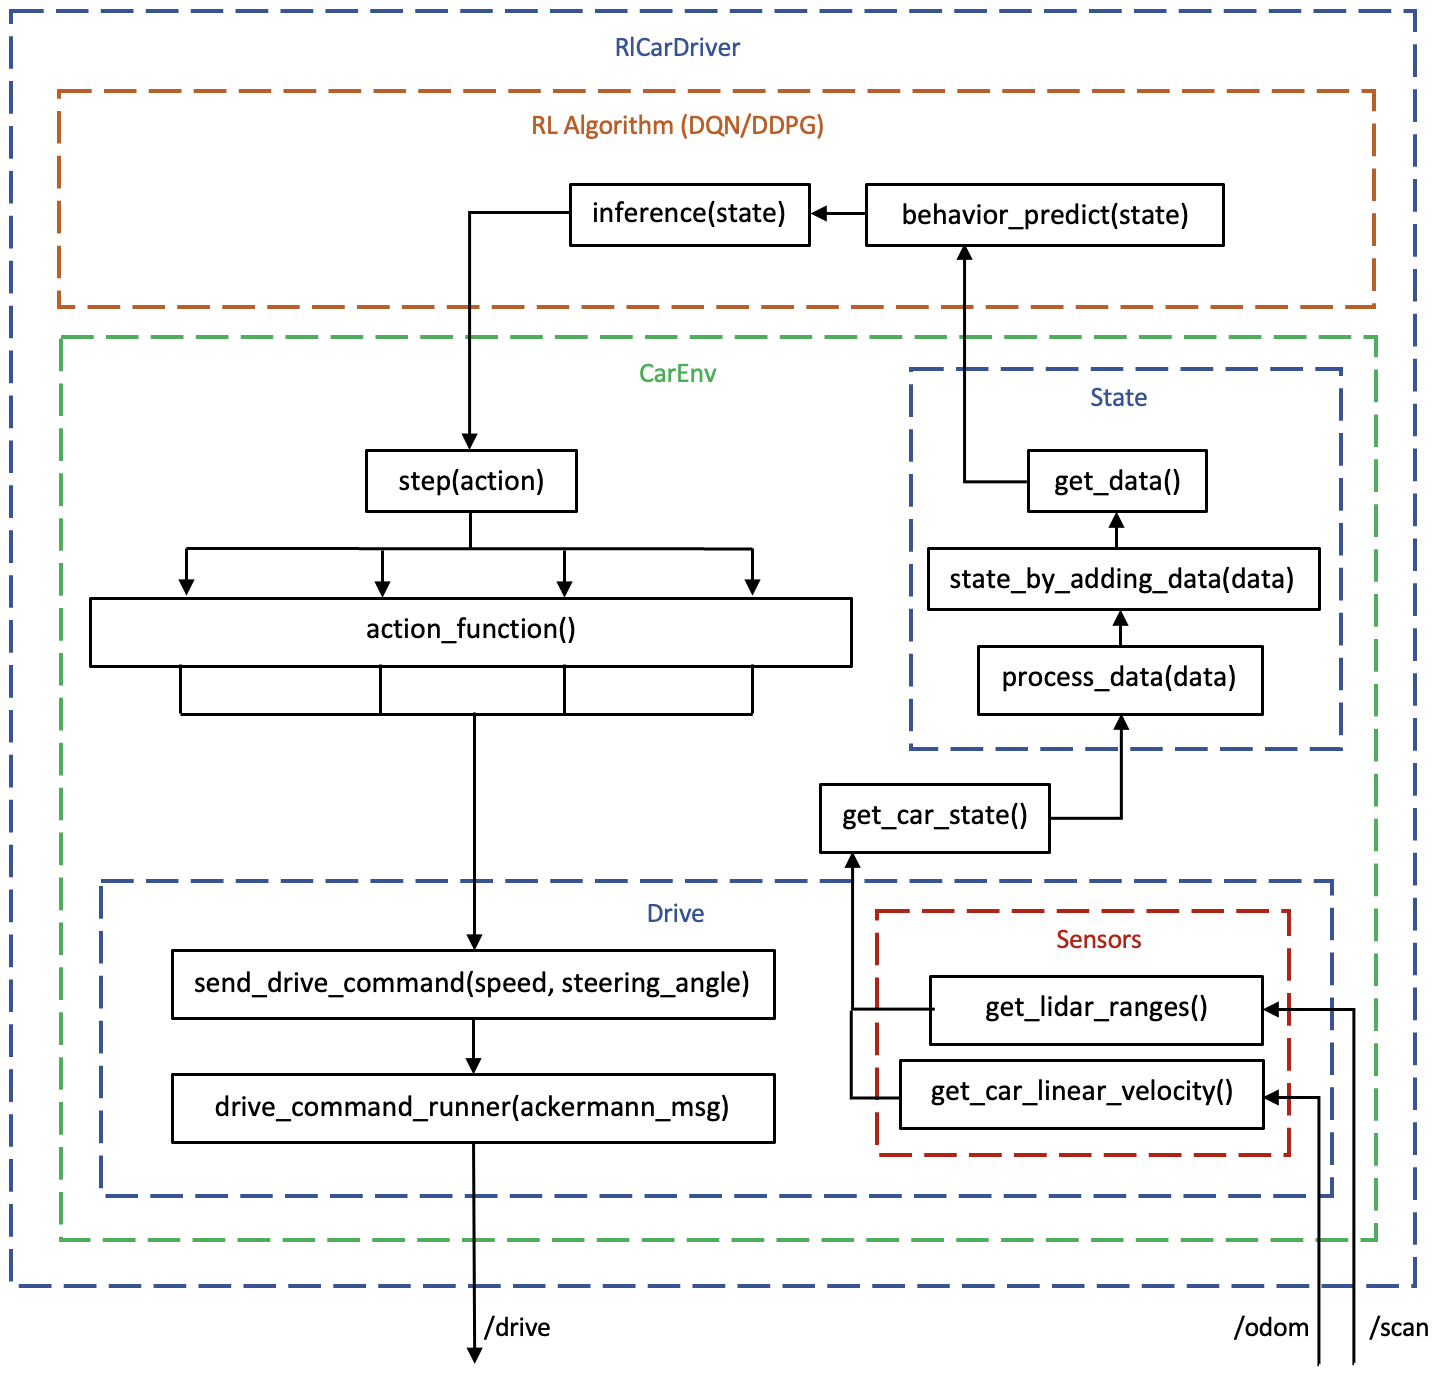
\includegraphics[scale=0.6]{Figures/inputs_outputs.png}
\caption{Functions involved in running an epoch and their inputs/outputs}
\label{inputs_outputs}
\end{figure}



Requirements E3, E5, E7 and E8 will be fulfilled using log files, listening to the \verb |/odom| topic to calculate the different metrics. For requirement E8 (Sim2Real gap assessment), the data will come from the Inertial Measurement Unit (IMU). \\

Several Python libraries will be used for the DQN and DDPG controllers:
\begin{itemize}
	\item TensorFlow 2.6.0: open source library with flexible architecture enabling high-performance computation for machine learning and deep learning applications
	\item Keras 2.7: a scalable framework built on TensorFlow offering simple deep learning implementations; it will be used to implement CNNs.
	\item Numpy: package providing high-performance computation capabilities for multi-dimensional arrays.
	\item Matplotlib 3.5.3: library offering visualisation tools.
\end{itemize}

A few non-functional software requirements will also be implemented (Table \ref{nonfuncsoreqtab}):

\begin{table}[H]
\centering
\begin{tabularx}{\textwidth}{||l|X|X|l||} 
 \hline
 Reference & Name & Description & Priority\\ [0.5ex] 
 \hline\hline
 N1 & Documentation & The different parameters used should be listed for reproducibility; instructions for running the code should be provided in a README file. & High\\
 \hline
 N2 & Compatibility & Instructions will be provided on how to run the controllers on other autonomous racing car platforms. & Low\\
  \hline
 N3 & Licensing & The use of the MIT License should be documented in the README file (Section \ref{legiss}). & Medium\\
  \hline
\end{tabularx}
\caption{Non-fuctional software requirements}
\label{nonfuncsoreqtab}
\end{table}


\section{Preliminary Investigations}
\label{preli}
To avoid encountering too many technical issues with the F1Tenth simulator and ROS, I have made several preliminary investigations: 
\begin{itemize}
	\item I have installed and tested the F1Tenth default simulator on my Ubuntu VM alongside ROS and Catkin.
	\item I have also found a way of installing the TensorFlow library on an ARM64 architecture by building the library from source. 
	\item I have also looked at how different maps can be imported in the simulator using the YAML format and editing the \verb |simulator_launch| file.
	\item I have looked at how I can make the ROS simulator run faster than real-time, which will be helpful when training the DQN and DDPG controllers; this is achievable using the \verb |/clock| topic with the \verb |/use_sim_time| parameter set to \verb |true|.
	\item I have looked at the ROS \verb|pid| module, that I could use to tune the parameters of the wall following controller.
\end{itemize}


These investigations have not directly answered any experimental or software requirements, but they will save time for the project's next steps.

\section{Evaluation}
\label{eva}

The goal was first to assess two different parameters: the speed and smoothness of the controller using the metrics introduced in Table \ref{table:1}; They are inspired by the metrics presented in \cite{benchmark}. They can all be measured directly from ROS topics, both in the F1Tenth simulator and on the actual car. The best-performing algorithm will be the one that maximises the average speed and minimises the other metrics.

\begin{table}[H]
\centering
\begin{tabularx}{\textwidth}{||l X||}
 \hline
 Metric & Description\\ [0.5ex]
 \hline\hline
 $T_{avg}$ & Average time to complete a full lap \\
 $V_{avg}$ & Average speed over a full lap \\
 $V_{max}$ & Maximum speed reached \\
 $A_{avg}$ & Average acceleration \\
 $A_{max}$ & Maximum acceleration \\
 $D_{max}$ & Maximum deceleration \\ [1ex]
\hline
\end{tabularx}
\caption{First set of metrics for performance evaluation}
\label{table:1}
\end{table}

After some consideration, it was decided to update the metrics to make them more relevant to the evaluation of the controllers (Table \ref{updatedmetrics}). Firstly, the average speed was removed as it is redundant with the time required to complete a lap, and the maximum reached speed was removed as it is always equal to the car's max speed. Secondly, the average positive and negative accelerations were introduced to replace the average acceleration, which is almost equal to 0. Finally, the average minimum LiDAR range was introduced to better assess the controller's safety, with higher values meaning that the controller is, on average, further away from the closest obstacle. \\

\begin{table}[H]
\centering
\begin{tabularx}{\textwidth}{||l X||}
 \hline
 Metric & Description\\ [0.5ex]
 \hline\hline
 $T_{avg}$ & Average time to complete a full lap \\
 $A_{avg}$ & Average acceleration \\
 $D_{avg}$ & Average deceleration \\
 $A_{max}$ & Maximum acceleration \\
 $D_{max}$ & Maximum deceleration \\
 $LiDAR_{min}$ & Average minimum LiDAR distance \\ [1ex]
\hline
\end{tabularx}
\caption{Updated set of metrics for performance evaluation}
\label{updatedmetrics}
\end{table}

I will consider this project to have successfully answered the research questions introduced in Section \ref{researchquestions} if:
\begin{itemize}
	\item The controllers implemented have been compared using the metrics from Section \ref{metricssection}, their ability to generalise to new race tracks and the training time required.
	\item The controllers have been compared when looking at the Sim2Real gap using the metrics from Section \ref{metricssection}.
\end{itemize}

I will consider the software part of the project successful if all the high and medium-priority functional and at least some of the non-functional software requirements are implemented.

